\documentclass{report}
\usepackage{graphicx}
\usepackage{wrapfig}
\usepackage{color}
\usepackage[usenames,dvipsnames]{xcolor}



\begin{document}

\title{\textbf{Homework 1:} Numerical Integration, differentiation, and bisection}
\author{A.L. Phillips II\\
  Department of Physics,% Astronomy, and Applied Physics,\\
  Rensselaer Polytechnic Institute\\
  \texttt{philla3@rpi.edu}}
\date{12 February 2013}
\maketitle
\chapter{Integration, differentiation, and root search}

\section{Sources of Error}
\begin{enumerate}
\item Roundoff vs Truncation
\\
\\Before entering a discussion on specific numerical methods, it is important to first discuss the types and affects of error upon such methods. Two sources of error affecting numerical methods are Round-off and Truncation errors. Round-off errors are the result of systems having a finite quantity of significant figures to represent numbers. For example, if a computer is capable of storing three significant figures, then it could approximate $ \frac{1}{3}$ as $0.333$. Because the computer is not representing $ \frac{1}{3}$ $exactly$ as $0.\overline{3}$, a round-off error ($\xi_{max_{T}}$) occurs. 
\\In the above case, $\displaystyle \xi_{max_{T}} = \frac{1}{3} - 0.333 = 0.000\overline{3} $
\\
\\Truncation error is the result of truncating (shortening) a mathematical procedure. The truncating of an operation can occur in various circumstances, e.g. whenever we are required to approach zero (integrate/differentiate) or use an infinite number of terms (a series expansions). For example, the Maclaurin series of $cos(x) = 1 - \frac{1}{2}x^2 + \frac{1}{24}x^4 - \frac{1}{720}x^6 + \ldots$ .Since we must chose a finite number of terms, a truncation error will ultimately result. If we choose two terms, the truncation error would then equal the sum of all the excluded terms. Namely, $\frac{1}{24}x^4 - \frac{1}{720}x^6 + \ldots$.  
\\
\end{enumerate}

\section{Numerical Integration Techniques}
\begin{enumerate}
\item Trapezoidal Method:
\\
\\
The trapezoid method calculates the area under a curve much like a Riemann sum. Here, rather than using rectangles, the trapezoid rule employs trapezoids (one pair of parallel sides). The graphic below depicts the use of a single trapezoid to approximate the area under the blue curve. The more intervals that ($b-a$) is subdivided into, the closer the "secant-shaped" tops of each trapezoid will approximate the tangent on the curve above it.\\
\\
. \hspace{30 mm} 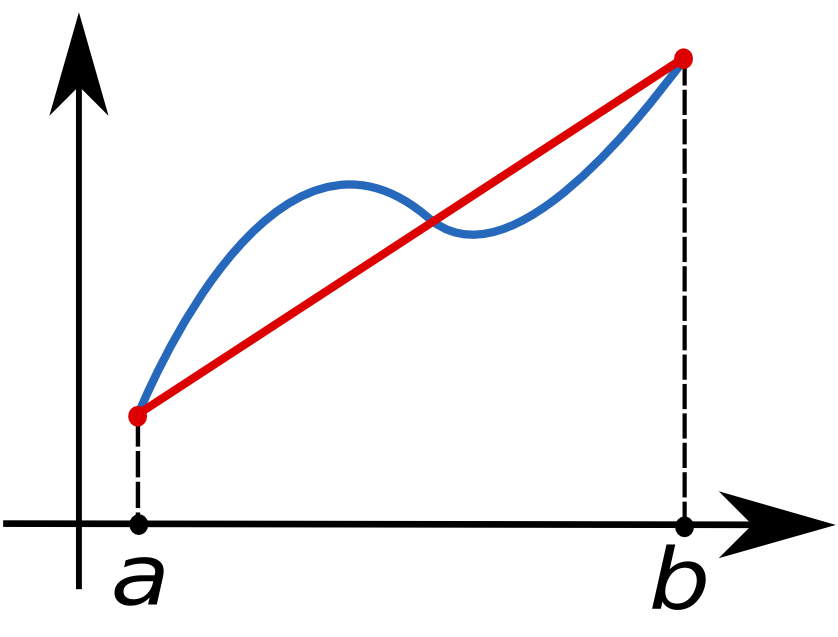
\includegraphics[scale=.15]{trapezoid.png}
\\
The Trapezoid Rule for approximating a definite integral is as follows:
\\ $\displaystyle \int^b_a f(x)\,dx  \approx  \frac{\Delta x}{2}\Big[f(x_{0})+2f(x_1)+\ldots+2f(x_{n-1})+f(x_n)\Big]$ 
\\where \hspace{10 mm} $\displaystyle \Delta x = \frac{(b-a)}{n}$ 
\hspace{7 mm} and \hspace{7 mm} $\displaystyle x_i = a + i(\frac{b-a}{n})$
\\
\\
\\Trapezoidal Error: 
\\
\\
When numerically computing $\displaystyle\int^5_1x^2\,dx$, the number of subdivision that the interval is broken into will vary the accuracy of the calculated area. The below graphic shows the relative error ($\epsilon = \frac{\left|experimental - known\right|}{known}$) as a function of the number of intervals.
\\.\hspace{10 mm} 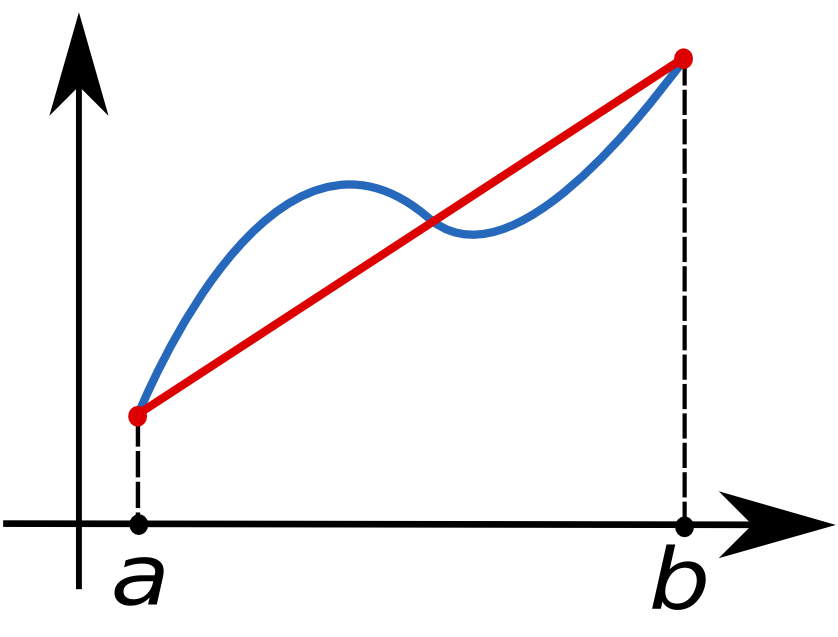
\includegraphics[scale=.95]{trapezoid.eps}
\\The maximum amount of truncation error ($\xi_{max_{T}}$) for the trapezoid method may be determined as follows:
\\
\\
. \hspace{30 mm} $\displaystyle \xi_{max_{T}} = \frac{(b-a)^{3}\left|f^{(2)}_{(max)}\right|}{12n^2}$  
\\
\\
\\Here,  $\displaystyle b$ and $\displaystyle a$ are the upper and lower limits of integration, $\displaystyle n$ is the number of intervals that ($b-a$) is divided into and $f^{(2)}_{(max)}$ is the second derivative of the function. The $(max)$ subscript indicates that the second derivative should be evaluated at the point in $\displaystyle [a,b]$ which maximizes the value of $f^{(2)}$.
\\
\\
\\Similarly, the minimum number of intervals needed to approximate an integral to within a given accuracy ($\xi_{max}$) may be determined by solving the above equation for $\displaystyle n$: 
\\
\\
. \hspace{30 mm} $\displaystyle n \geq \sqrt{\frac{(b-a)^{3}\left|f^{(2)}_{(max)}\right|}{12(\xi_{max})}} $
\\
\\Note: $\displaystyle n$ must be a whole number; therefore if $n \geq 10.5$ then choose $n = 11$
\\
\\
\item Simpson's Rule:
\\
\\
Simpson's rule also calculates the area under a curve similar to a Riemann sum. Here, rather than using rectangles, Simpson's rule employs parabolas for the "rectangles" top. The graphic below depicts the use of a red parabola between two intervals to approximate the area under the blue curve. The more intervals that are added between $a$ and $b$, the closer the "parabolic-shaped" tops of each interval will become to the tangent on the curve above it.
\\. \hspace{30 mm} 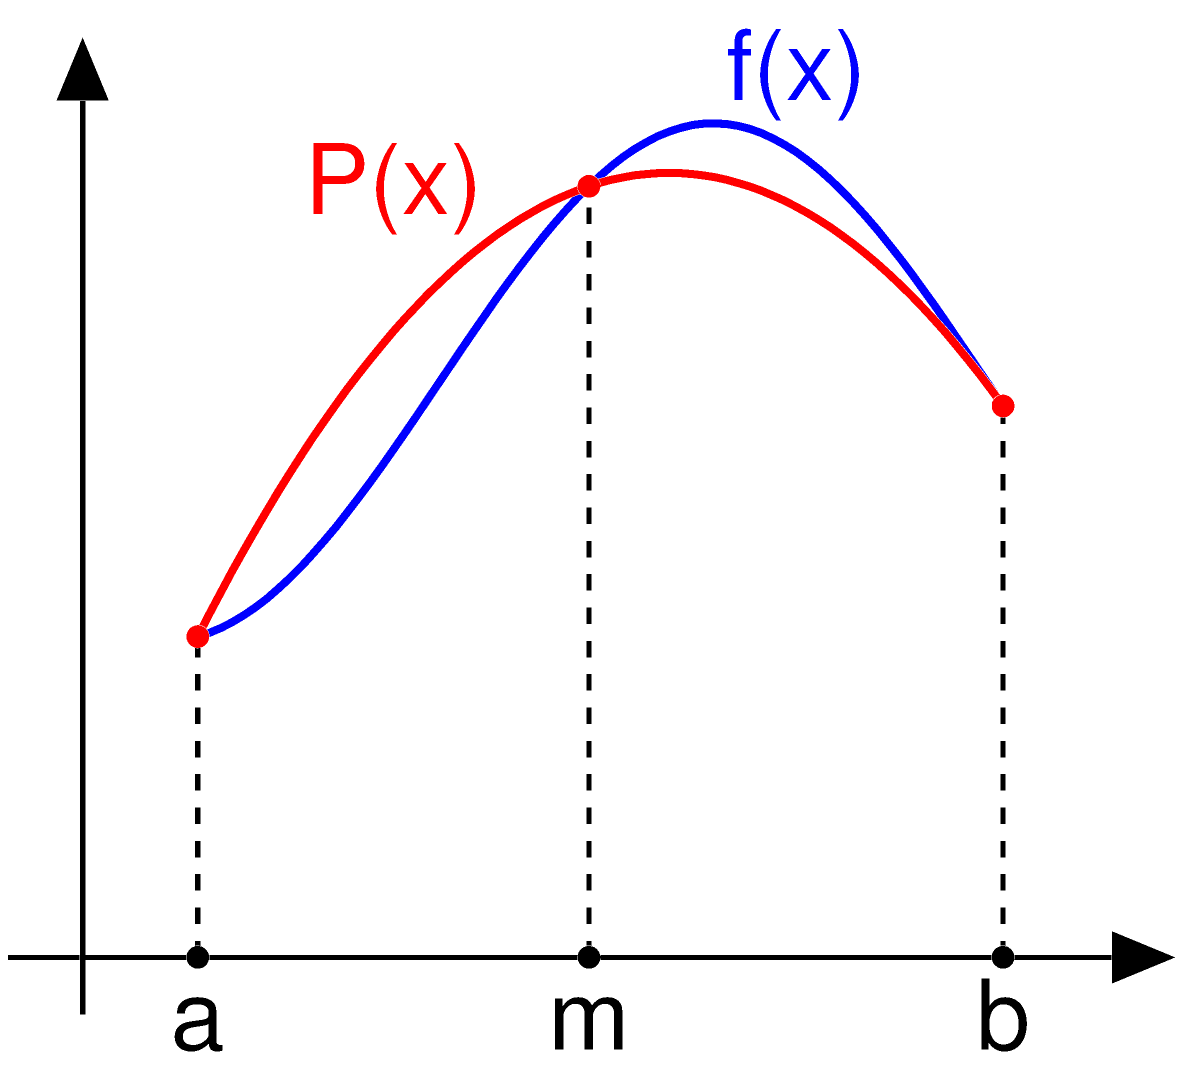
\includegraphics[scale=.10]{simpson.png}
\\
\\
\\
The formula for calculating Simpson's Rule is as follows:
\\
\\ $\displaystyle \int^b_a f(x)\,dx  \approx  \frac{\Delta x}{3}\Big[f(x_{0})+4f(x_1)+2f(x_2)+4f(x_3)+\ldots+2f(x_{n-2})+4f(x_{n-1})+f(x_n)\Big]$, \hspace{4 mm} where $\displaystyle \Delta x = \frac{(b-a)}{n}$ 
\hspace{7 mm} and \hspace{7 mm} $\displaystyle x_i = a + i(\frac{b-a}{n})$
\\
\\Note: Simpson's Rule requires an even number of intervals $(n)$. 
\\
\\
\\Simpson Rule Error: 
\\
The accuracy of numerically computing $\displaystyle\int^5_1x^2\,dx$ will vary with the number of intervals used. The below graphic shows the relative error ($\epsilon$) of both (\textcolor{red}{Simpson's Rule}) and the (\textcolor{blue}{Trapezoid Method}) as a function of interval quantity.
\\
\\.\hspace{10 mm} \includegraphics[scale=.95]{trapezoidsimpson.eps}
\\
\\Notice how quickly Simpson's rule converges versus the Trapezoid Rule. This is due to Simpson's use of a parabolic curve to approximate the area under $x^2$ (a parabola). Here, because the tool used to approximate the curve is the same as the curve itself, the approximation may be exact. Conversely, were we integrating a linear function, then the trapezoid method would be optimal due to its use of secant lines.
\\
\\The maximum amount of truncation error ($\xi_{max_{T}}$) for Simpson's Rule may be determined as follows:
\\
\\
. \hspace{30 mm} $\displaystyle \xi_{max_{T}} = \frac{(b-a)^{5}\left|f^{(4)}_{(max)}\right|}{180n^4}$ 
\\
\\
\\
\\
\\The minimum number of intervals needed to approximate an integral to within a given accuracy ($\xi_{max}$) may be determined by isolating $\displaystyle n$ from the equation above: 
\\
. \hspace{30 mm} $\displaystyle n \geq \sqrt[4]{\frac{(b-a)^{5}\left|f^{(4)}_{(max)}\right|}{180(\xi_{max})}} $
\\
\\Note: For Simpson's Rule, $\displaystyle n$ must be an even and whole number
\\
\\
\item Three-Point Gaussian Quadrature (GQ):
\\
\\Gaussian Quadrature is another numerical integration method. Of the previous methods discussed, GQ is capable of obtaining the most accurate approximations (often exact). In the case where GQ, FDD, CDD have equivalent accuracy, GQ is found to have required fewer intervals. This is done by evaluating $f(a)$ at a chosen abscissas. The abscissas is found by determining the roots of an orthogonal polynomial which has the same interval and weight. GQ is the preferred method of integration due to its ability to exactly fit any n-degree polynomial.
\\
\\
\\The formula for three-point Gaussian Quadrature is as follows:
\\
\\$\displaystyle \int^b_a f(x)\,dx  \approx c_1f(x_1)+c_2f(x_2)+c_3f(x_3)$, where 
\\$x_1=-0.7746, x_2=0, x_3=0.7746$ and weights $c_1=0.555\overline{6}, c_2=0.888\overline{9} and c_3=0.555\overline{6}$
\\
\\Note: GQ is not limited to only three-point calculations. 
\end{enumerate}


\section{Numerical Differentiation Techniques}
\begin{enumerate}
\item Forward Divided Difference (FDD)
\\
\\
Forward difference is a numerical method of differentiation. It employs the familiar limit definition of a derivative but it substitutes ($\Delta x \rightarrow 0$) with a finite step size ($h$). The forward difference formula is as follows:
\\
\\
. \hspace{7 mm} $\displaystyle f'(x) \approx \frac{f(x+\Delta x)-f(x)}{\Delta x}$ where $\Delta x$ is a finite term ($h$).
\\
\\
\\
\\
FDD Error:
\\
\\Because ($\Delta x \rightarrow 0$) is approximated by a finite step size ($h$), a truncation error will result. To minimize the truncation error, $h$ should be taken sufficiently small. However, there is a computational limit to how small $h$ can be. Machine Epsilon ($\epsilon$) is the largest number that when added to another number, does not change the other number. That is, it is the smallest representable number that is not zero. Note there is no universal $\epsilon$. Machine epsilon is specific to both a systems architecture and the data structure being used. Each system and specific data type will have it's own epsilon. In my case, my machine epsilon ($\epsilon$) for a double is $\approx$ $2.22045\times10^-16$. 
\\
\\FDD Considerations:
\\
\\ Let us consider the relative error of allowing $\Delta x = h = \epsilon$
\\
\\
. \hspace{15 mm} $\displaystyle f_{FDD}'(\epsilon) \approx \frac{f(x+\epsilon)-f(x)}{\epsilon} \approx \frac{f(x)-f(x)}{\epsilon} \approx \frac{0}{\epsilon} \approx 0$
\\ 
\\
\\. \hspace{15 mm}$\displaystyle\xi_{max} \approx \frac{\left|f_{FDD}'(\epsilon)-f'(x)\right|}{f'(x)} \approx \frac{\left|0-f'(x)\right|}{f'(x)} \approx 1$ 
\\. \hspace{15 mm} Note: $f'(x)$ is the exact analytical derviative.
\\
\\Notice that if $h$ is chosen to be $\geq \epsilon$ then $\xi_{max}$ will be $\geq 1$. Therefore, to minimize error, and thereby maximize accuracy, an $h$ should be chosen such that the truncation error and round-off error are approximately the same.
\\
\\The following $LogLog$-plot depicts the relative error($\epsilon$) versus step size ($h$) of the FDD approximations for: $x^2(\textcolor{blue}{blue})$, $x^3(\textcolor{red}{red})$, $e^{-x}(\textcolor{green}{green})$ and $sin(x)ln(x)(\textcolor{brown}{brown})$
\\
\\
\\.\hspace{6 mm} 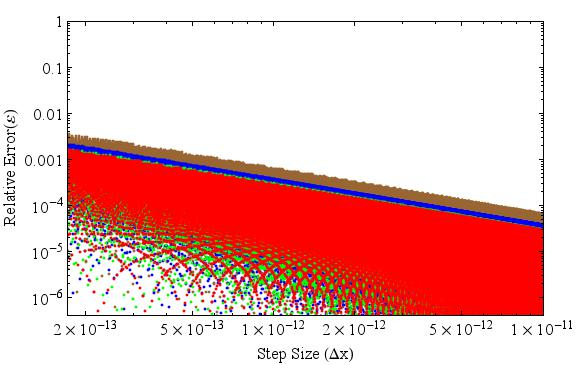
\includegraphics[scale=.5]{forwardDiff.jpeg}
\\
\\
\\
\item Central Divided Difference (CDD)
\\
\\The Central Difference is similar to FDD except that CDD is evaluated at half of the step size. Due to this, CDD has an additional order of accuracy for smooth functions. The Central Fifference formula is as follows:
\\
\\
\\$\displaystyle f'(x) \approx \frac{f(x+\Delta x)-f(x)}{2\Delta x}$ where $\Delta x$ is a finite term ($h$).
\\
\\
\\\\The following $LogLog$-plot depicts the relative error($\epsilon$) versus step size ($h$) of the CDD approximations for: $x^2(\textcolor{blue}{blue})$, $x^3(\textcolor{red}{red})$, $e^{-x}(\textcolor{green}{green})$ and $sin(x)ln(x)(\textcolor{brown}{brown})$
\\
\\.\hspace{6 mm} 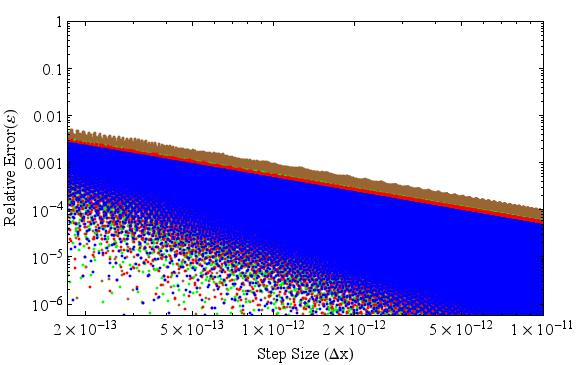
\includegraphics[scale=.5]{centralDiff.jpeg}
\\\item Five Point Stencil (FPS)
\\The formula for the FPS method is as follows:
\\
\\$\displaystyle f'(x) \approx \frac{-f(x+\Delta x)+8f(x+\Delta x)-8f(x-\Delta x)+f(x-2\Delta x)}{12\Delta x}$ 
\\where $\Delta x$ is a finite term ($h$).
\\
\\The truncation error due to FPS may be estimated as follows:
\\
\\.\hspace{25 mm}$\xi_{max} = f'(x)-\frac{1}{30}f^5(x)h^4+O(h^5)$
\\\\The following $LogLog$-plot depicts the relative error($\epsilon$) versus step size ($h$) of the FPS approximations for: $x^2(\textcolor{blue}{blue})$, $x^3(\textcolor{red}{red})$, $e^{-x}(\textcolor{green}{green})$ and $sin(x)ln(x)(\textcolor{brown}{brown})$
\\\\.\hspace{6 mm} 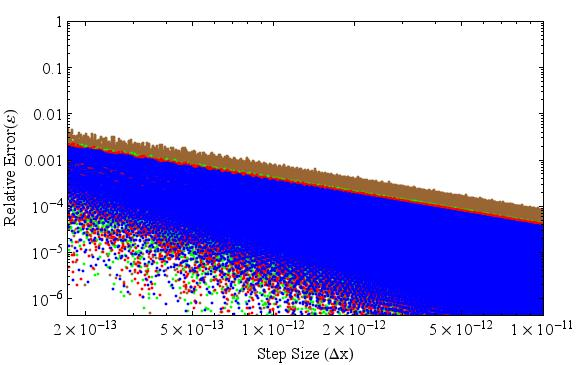
\includegraphics[scale=.5]{fivePoint.jpeg}
\end{enumerate}
\section{Methods of Root Finding}
\begin{enumerate}
\item The Bisection Method
\\
\\The bisection method is an algorithm which can pinpoint the root of most functions. Several conditions must be satisfied in order for the method to prove successful. First, the user must have determined an approximate location for the root. This is necessary because the algorithm requires an interval whose upper and lower bound must contain the root. The principle function must also be real, continuous (within the interval) and have opposite signs at the initial upper and lower bounds as depicted below. If these preconditions are met, the bisection is guaranteed to converge on a root.
\\
\\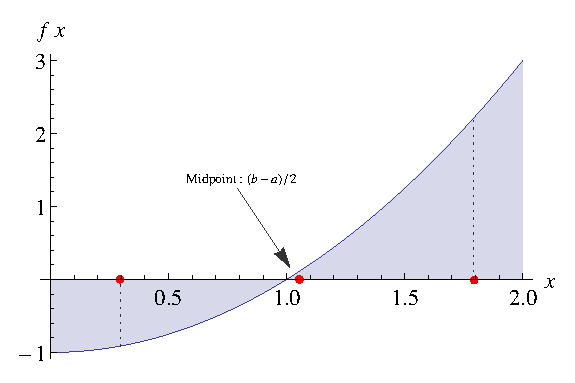
\includegraphics[scale=1.3]{bisection.eps}
\\
\\Algorithm:  
\\
\\The method is implemented by recursive comparison of the sign of the function at a specified lower (or upper) boundary with the sign of the function at a calculated midpoint between the upper and lower boundaries. If the product of the signs are negative, then the midpoints value is assigned to the the upper boundary and a new midpoint is calculated for the next iteration. If the product of lower bound and the newly calculated midpoint is positive, then the value of midpoint is assigned to the lower boundary and another midpoint is calculated for the next iteration. This process is repeated until the product of the lower bound and the midpoint is $0$. The zero product indicates discovery of the root: $f(midpoint)=0$.
\\
Considerations: 
\\
\\While the bisection method is guaranteed to work, its preconditions are stringent and its application may be limited for certain functions. For example, $f(x)=x^2$. Here, since the function is $\geq0$ $\forall x$, the bisection methods preconditions cannot be satisfied. The precondition are unmet because the value of the function at the initial boundaries have identical signs. By definition, the bisection method requires opposite signs and so the routine goes uninitialized.
\\
\\ Depending on the choice of boundaries, bisection can require excessive iterations. If one of the boundaries is chosen sufficiently close to the root while the other is not, it will take many iterations before of $\frac{\left|upper-lower\right|}{2}$ before the algorithm can converge. The number of iterations increase as ($upper$) is chosen further from the root and ($lower$) is chosen closer.  
\\
\\The maximum error of the bisection method may be controlled by the initial selection of the boundaries. That is, the true error can be no larger then $(upper-lower)$. Due to the implementation of the midpoint, the error is halved for each iteration. 
\\
\item The Newton Raphson Method (NRM)
\\
\\The Newton Raphson method is an algorithm which is capable but not guaranteed to locate the root of most functions. Unlike the bisection algorithm with its many preconditions, NRM requires only a single guess (seed) from the user and generally requires less iterations to converge at a root.
\\
\\Algorithm:  
\\
\\NRM is implemented by recursively comparing positions on the x-axis until the relative error between them meets some user specified tolerance or maximum number of iterations. The method is depicted as follows:
\\
\\
\\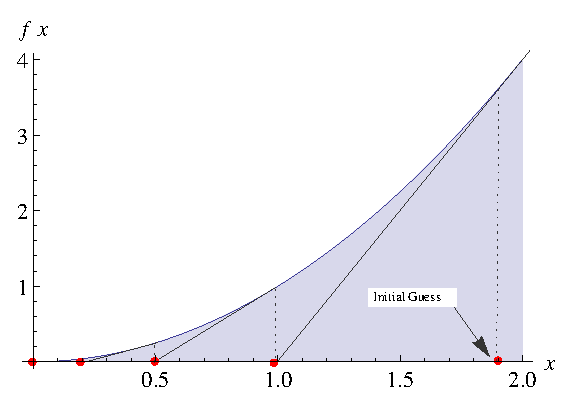
\includegraphics[scale=1.2]{newtonraphson.eps}
\\
\\The initial guess is the first point ($x_0$). It is provided as a seed by the user from which the method begins its search. To determine the second point, the tangent of the function at $f(x_0)$ is extended out to $x_1$ on the x-axis. 
\\.\hspace{30 mm} Here, $\displaystyle x_1 = x_0 - \frac{f(x_0)}{f'(x_0)}$  
\\
\\ The above process is repeated until a specified number of iterations are reached or the relative error between two points, $\displaystyle \xi = \frac{\left|x_1-x_0\right|}{x_1}$, is less then a specified accuracy. Once the maximum iterations or accuracy are met, $x_i$ is determined to be the root.
\\
\\
\\Considerations: 
\\
\\While NRM requires little input from the user, it does not guarantee convergence on any or all roots of a function. For example, note in the depictions below, how $x^2+2$ may diverge or $sin(x)$ may fail to discover all roots:
. \hspace{4 mm} 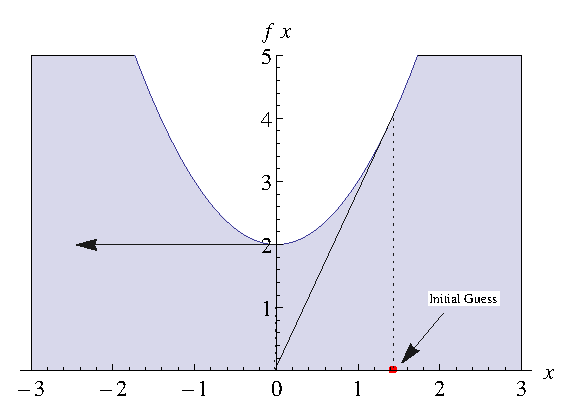
\includegraphics[scale=.5]{divergence.eps} 
\hspace{6 mm}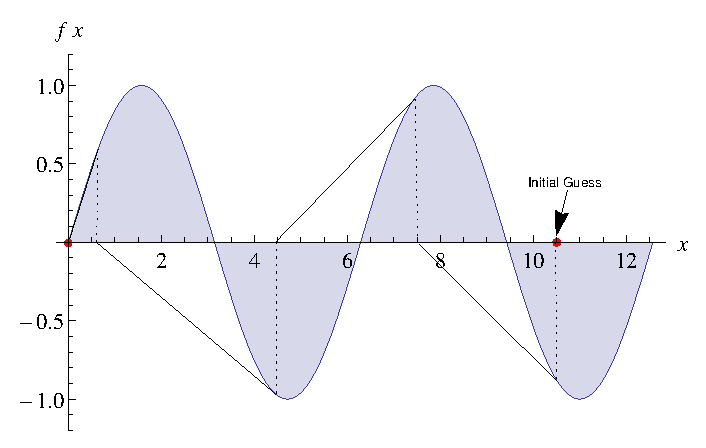
\includegraphics[scale=.5]{rootskipping.eps}
\end{enumerate}

\end{document}
